The vector form of the equation is 
\begin{align}
\vec{x}^T\myvec{3&0\\0&0}\vec{x}+\myvec{-2\sqrt{6}&0}\vec{x}+2 = 0
\end{align}

The values of $\vec{x}$ are found in the following python code
\begin{lstlisting}
solutions/6/codes/conics/example/conics.py
\end{lstlisting}

$\vec{x}=\myvec{0.81649658\\0}, \myvec{0.81649658\\0}$ \\
which can be verified from  Fig. \ref{fig:5.1.6_parabola} 
generated by the following python code 
\begin{lstlisting}
codes/conics/example/conics.py
\end{lstlisting}
\begin{figure}[!ht]
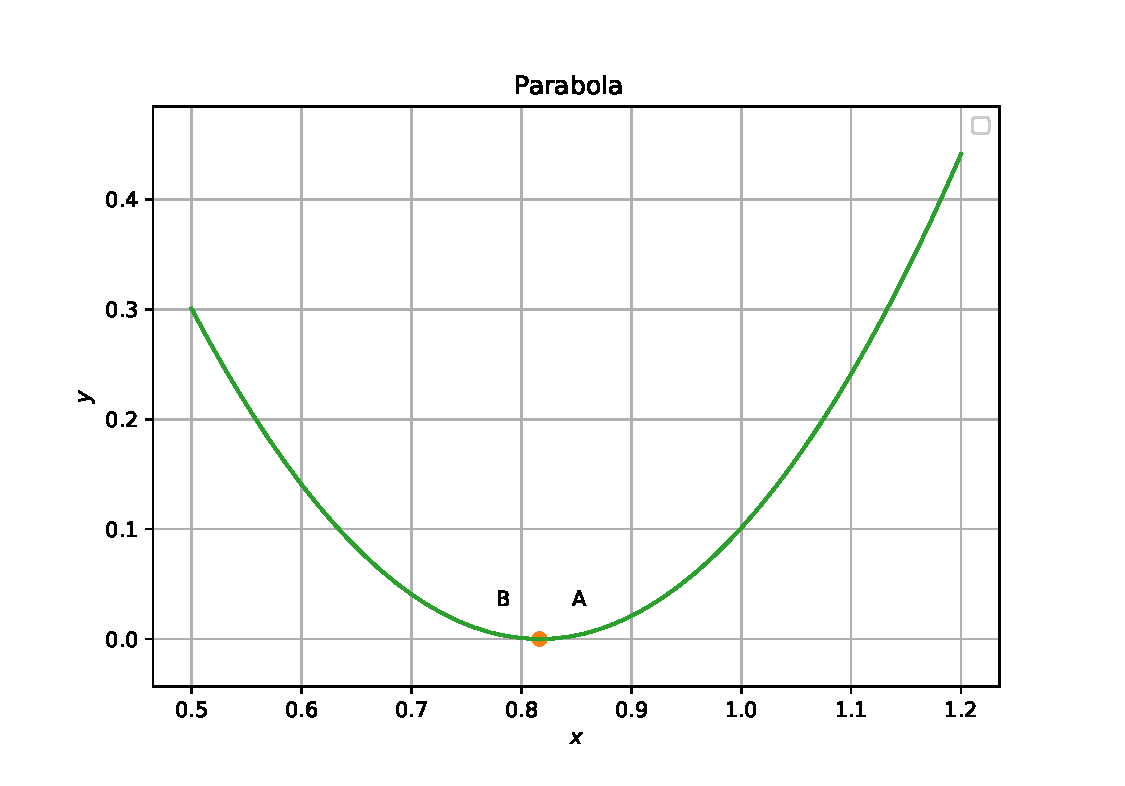
\includegraphics[width=\columnwidth]{./solutions/6/codes/conics/example/conics.eps}
\caption{Parabola}
\label{fig:5.1.6_parabola}
\end{figure} 
